\documentclass{article}
\usepackage{spconf,amsmath,amssymb,graphicx,booktabs,url}
\usepackage[T1]{fontenc}
\usepackage{times}
\usepackage[hidelinks]{hyperref}
\hypersetup{pdftitle={Same Image, Different Coverage: Auditing Batch-Adaptive Medical Classifiers},pdfauthor={Shivam Gupta},pdfsubject={Medical image classification, batch normalization, and conformal prediction}}
\title{Same Image, Different Coverage:\\Auditing Batch-Adaptive Medical Classifiers}
\name{Shivam Gupta}
\address{Independent Researcher, India\\\texttt{shivam1720406@gmail.com}}
\newcommand{\PneuContextMean}{92.9\%}
\newcommand{\PneuContextJoint}{85.5\%}
\newcommand{\PneuCMRJoint}{96.6\%}
\newcommand{\PneuEnvelopeJoint}{96.1\%}
\newcommand{\PneuCMRSize}{1.68}
\newcommand{\PneuEnvelopeSize}{1.90}
\newcommand{\PneuContextSize}{1.28}
\newcommand{\FlipRange}{13.1--51.0\%}
\newcommand{\PneuGapCI}{7.5 [5.9, 9.2]}
\begin{document}
\ninept
\maketitle
\begin{abstract}
Prediction-time batch normalization makes a medical classifier's output depend on its batch companions. We audit whether prediction-set coverage for an unchanged query survives companion replacement. Three medical imaging benchmarks, batch- and group-normalized architectures, and five training seeds compare average context coverage with true-label inclusion under every fixed context. A 224-pixel pretrained ResNet18 extension tests a higher-resolution setting. On PneumoniaMNIST, context-specific calibration of the compact residual model gives \PneuContextMean\ mean coverage but \PneuContextJoint\ simultaneous coverage. We compare established simultaneous conformal corrections and their coverage--size trade-offs. Duplicate checks, lesion-disjoint dermatology partitions, and calibration-split sensitivity support reproducibility. The findings motivate explicit companion-context assumptions for calibrated medical-image inference services.
\end{abstract}
\begin{keywords}
medical imaging, batch normalization, conformal prediction, deployment audit
\end{keywords}

\section{Introduction}
A hospital inference service may form a batch from the studies currently in a queue. With prediction-time batch normalization (BN), changing the other studies changes a query's normalized features even if its pixels remain identical. Prediction-time BN can improve robustness under covariate shift \cite{nado}, but class imbalance and problematic companion samples are established failure modes \cite{delta,medbn}. For a system returning a set of plausible diagnoses, a separate question arises: does its true-label inclusion claim survive alternative companion contexts?

Standard split conformal prediction protects an exchangeable future example for a specified scoring procedure \cite{angelopoulos}. It does not equate average coverage across inference contexts with inclusion for the \emph{same} example under all contexts. This distinction matters when a service advertises a coverage level while its scheduler may change batch membership. We study the distinction by holding model weights and query pixels fixed and replacing only companions.

This study contributes a paired audit separating class changes, mean context coverage, and simultaneous coverage; a comparison of established conformal corrections on identical predictions; and a reproducible three-benchmark evaluation with five training seeds, normalization controls, duplicate checks, and calibration-split sensitivity. The contribution is the operational audit; the normalization and conformal methods are established. Code, weights, and per-image outputs are released.\footnote{\url{https://github.com/shi1720/medical-batch-coverage-audit}}

\section{Related work}
BN \cite{bn} couples examples through estimated moments. Prediction-time BN \cite{nado}, TTN \cite{ttn}, DELTA \cite{delta}, and MedBN \cite{medbn} address adaptation, mixed moments, imbalance, and adversarial companions. Our intervention uses unchanged, unoptimized training images and freezes all learned parameters; it is not a reproduction of entropy-minimizing or continually updated adaptation.

Robust conformal prediction already calibrates restrictive scores over perturbations \cite{massena}. Max-Rank \cite{maxrank} exploits dependence for simultaneous control; we implement its finite-sample-corrected score-space version \cite{corrected}. Batch conformal classification \cite{gazin} concerns multiple queried examples, whereas our joint event concerns one query under several contexts. Medical VLM adaptation with conformal prediction is also established \cite{scpt,lata}. Event reordering can also alter adaptive ECG conformal thresholds without changing signals or classifier outputs \cite{conformalshift}. Here thresholds are stateless after calibration, and companion replacement changes classifier scores through BN. Our focus is the resulting all-context coverage estimand.

\section{Companion-context audit}
\subsection{Fixed intervention and estimands}
Let $f_\theta(x;B_j)$ be a trained $K$-class classifier evaluated on query $x$ with $b-1$ fixed companions $B_j$. Let $\mathcal B=\{B_1,\ldots,B_M\}$ be chosen from training data independently of calibration and evaluation examples. For each query, normalization uses the batch $\{x\}\cup B_j$. Query groups are isolated even during vectorized inference. Each context therefore defines a fixed score
\begin{equation}
 s_j(x,y)=1-[f_\theta(x;B_j)]_y.
\end{equation}
For thresholds $t_j$, write $C_j(x)=\{y:s_j(x,y)\le t_j\}$. We report
\begin{align}
 \widehat{\mathrm{Cov}}_{\rm mean}&=\frac1{NM}\sum_{i=1}^{N}\sum_{j=1}^{M}\mathbf1\{y_i\in C_j(x_i)\},\\
 \widehat{\mathrm{Cov}}_{\rm all}&=\frac1N\sum_{i=1}^{N}\mathbf1\{y_i\in\cap_j C_j(x_i)\}.
\end{align}
The second event requires true-label inclusion under every menu context. Its failures can affect different images across contexts even if each context is individually calibrated. Per-context marginal coverage $1-\alpha$ alone yields only the union-bound lower bound $\max(0,1-M\alpha)$ for the joint event, not $1-\alpha$.

\subsection{Calibration comparators and guarantee scope}
For calibration scores $a_1,\ldots,a_n$, let $Q_\alpha(a)$ be the $\lceil(n+1)(1-\alpha)\rceil$th ascending value, using $+\infty$ when the rank exceeds $n$. We compare: \emph{nominal}, which calibrates $s_1$ under the first natural context and reuses that threshold; \emph{context-specific}, $t_j=Q_\alpha(s_j)$; \emph{Bonferroni}, $t_j=Q_{\alpha/M}(s_j)$; \emph{Corrected Max-Rank} (CMR) \cite{corrected}; and a \emph{score envelope}, $t_j=q$ for every $j$, where
\begin{equation}\label{eq:envelope}
 S(x,y)=\max_j s_j(x,y),\qquad q=Q_\alpha\big(\{S(x_i,y_i)\}_{i=1}^n\big).
\end{equation}
For CMR, compute maximum-tie ranks within each context, take $r=Q_\alpha(\{\max_j R_{ji}\}_i)$, and set $t_j$ to context $j$'s $(r+1)$st ascending calibration score, or $+\infty$. The additional order statistic follows \cite{corrected}. Maximum-tie ranks and closed thresholds give a conservative tie extension, detailed in the reproducibility notes.

For a fixed model and menu, if calibration examples and the future query are exchangeable, the envelope satisfies
\begin{equation}
 \Pr\{Y\in C_j(X)\ \text{for all }j\}\ge1-\alpha.
\end{equation}
Indeed, the simultaneous event equals $S(X,Y)\le q$; the usual exchangeable-rank argument applies to this scalar score. This applies existing robust split conformal prediction \cite{massena}. The probability is marginal over calibration and query, conditional on the fixed model/menu, not conditional on a particular realized calibration set. It excludes unseen contexts, changing model state, and distribution shift. Each deployed $C_j$ needs one context pass; constructing the companion-independent intersection needs all $M$ passes. Mean deployed set size is the primary efficiency metric. Empty sets are allowed; empty/singleton rates and intersection sizes are released.

\section{Experiments}
\subsection{Data integrity and protocol}
We use 28-pixel PneumoniaMNIST, BreastMNIST \cite{medmnist,kermany,breast}, and the published DermaMNIST-C correction \cite{dermac,ham}. Tasks are chest-radiograph pneumonia classification, ultrasound malignancy classification (normal/benign merged), and seven-class dermoscopic lesion classification. A label-blind SHA-256 audit removes exact image-byte duplicates with training, then validation, then test priority. Original PneumoniaMNIST has eight distinct train--validation overlaps; BreastMNIST has one train--test overlap. The correction's dermatology partitions are lesion-disjoint, verified using metadata. One image per test lesion is retained in metadata order before calibration splitting. Table~\ref{tab:data} gives final counts. Patient identifiers are unavailable for these experiments; lesion separation and exact-byte removal do not establish patient independence.

\begin{table}[t]
\centering
\caption{Final disjoint image counts; dermatology test units are distinct lesions. Calibration/evaluation halves use seed 20406.}
\label{tab:data}
\begin{tabular}{lrrrr}\toprule
Dataset & Train & Val. & Cal. & Eval.\\\midrule
PneumoniaMNIST & 4690 & 516 & 310 & 311\\
BreastMNIST & 546 & 78 & 77 & 78\\
DermaMNIST-C & 8213 & 573 & 574 & 575\\\bottomrule
\end{tabular}
\end{table}

Primary models are a three-block CNN-BN (16/32/64 channels), a compact residual BN model (16/32/64 channels), and an otherwise matched CNN with four-group GroupNorm \cite{gn}. We train five seeds, AdamW (learning rate $10^{-3}$, weight decay $10^{-4}$), batch 64, for 25 epochs without augmentation; the lowest validation negative log likelihood selects a checkpoint. Inputs are $x/127.5-1$. All training uses two CPU threads; vectorized inference uses Apple MPS, checked against CPU. We use population variance for current-batch inference, matching PyTorch training-mode BN with frozen affine parameters and no running-state updates.

A secondary 224-pixel PneumoniaMNIST extension fine-tunes ImageNet-pretrained ResNet18 \cite{resnet}, all parameters, for five epochs on MPS (five seeds, AdamW $10^{-4}$ learning rate and weight decay, batch 32, no augmentation, lowest validation NLL). Grayscale inputs are repeated across RGB and ImageNet-normalized. Source-image indices follow primary cleaning, with an additional 224-pixel byte audit. BN replacement preserves pretrained state. RN18-224 uses the same context design and conformal methods.

The batch contains one query and 15 companions. For each of three fixed draws (seeds 801--803), the menu contains a natural-frequency context, an approximately class-balanced context, and one homogeneous context per class: $M=12$ for binary datasets and $M=27$ for dermatology. Homogeneous contexts deliberately stress composition; labels are used to construct the audit menu, not supplied to inference or claimed available to a scheduler. Balanced draws are independent within each class and can repeat images; exact context indices are released. The same menu and unstratified calibration/evaluation split apply across models and seeds. Random partitioning supports image-level finite-pool analysis, without establishing exchangeability of future patients. We set $\alpha=0.1$ throughout.

The exploratory protocol and amendments are released. Exact-byte cleaning and the published dermatology correction preceded final training on the corresponding datasets; earlier pilots are excluded. Runtime motivated restricting mixed-moment, first-layer-only, matched affine-intensity, and batch-size controls to seed 0. CMR was added after the literature review. These choices are disclosed rather than described as preregistered. APS score sensitivity was added after the binary-dataset results. Repeated calibration splitting uses 100 fixed random splits of the same held-out pool; it measures split sensitivity, not 100 independent datasets.

\subsection{Results}
\begin{table*}[t]
\centering
\caption{Current-batch BN: simultaneous coverage (\%) / mean deployed set size. Each cell is the mean across five training seeds. Per-context calibration targets each context separately; simultaneous methods target the joint event. Full seed SDs, accuracy/AUC, and per-image outputs are released.}
\label{tab:main}
\begin{tabular}{llrrrrrr}\toprule
Dataset & Model & Flip (\%) & Nominal & Per-context & Bonferroni & CMR & Envelope\\\midrule
PneumoniaMNIST & CNN-BN & 16.2 & 85.1 / 1.19 & 90.9 / 1.19 & 99.4 / 1.77 & 92.5 / 1.23 & 92.2 / 1.33\\
PneumoniaMNIST & ResNet-BN & 41.4 & 63.5 / 1.16 & 85.5 / 1.28 & 99.3 / 1.73 & 96.6 / 1.68 & 96.1 / 1.90\\
BreastMNIST & CNN-BN & 13.1 & 83.6 / 1.14 & 85.9 / 1.13 & 100.0 / 2.00 & 91.5 / 1.26 & 92.8 / 1.48\\
BreastMNIST & ResNet-BN & 51.0 & 57.4 / 1.14 & 77.7 / 1.24 & 100.0 / 2.00 & 92.1 / 1.59 & 92.6 / 1.82\\
DermaMNIST-C & CNN-BN & 23.1 & 78.2 / 1.13 & 81.6 / 1.26 & 98.3 / 2.87 & 89.7 / 1.67 & 90.6 / 1.85\\
DermaMNIST-C & ResNet-BN & 28.2 & 73.7 / 1.12 & 77.0 / 1.36 & 98.4 / 3.07 & 90.4 / 2.00 & 89.7 / 2.36\\
PneumoniaMNIST & RN18-224 & 44.8 & 55.5 / 1.01 & 83.0 / 1.17 & 98.1 / 1.63 & 93.6 / 1.37 & 92.0 / 1.74\\
\bottomrule\end{tabular}
\end{table*}
\begin{figure}[t]
\centering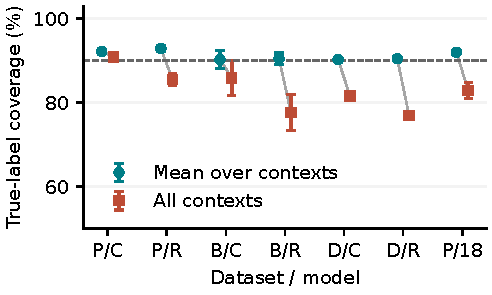
\includegraphics[width=\columnwidth]{figures/coverage.pdf}
\caption{Context-specific calibration: five-seed mean and simultaneous coverage (bars: seed SD). P/B/D: pneumonia/breast/dermatology; C/R: compact CNN/residual; 18: pretrained RN18-224. Dashed line: 90\% target.}
\label{fig:coverage}
\end{figure}
Table~\ref{tab:main} reports all primary BN configurations and the pretrained RN18-224 extension. The source-statistics and GroupNorm controls are exactly companion-invariant in saved probabilities. Under current-batch BN, changing companions produces \FlipRange\ class-flip rates across the six primary dataset--architecture settings. This is a paired intervention: the query itself is never perturbed.

The compact residual PneumoniaMNIST model illustrates why mean coverage is insufficient. Its context-specific mean coverage is \PneuContextMean, but simultaneous coverage is \PneuContextJoint. The paired difference is \PneuGapCI\ percentage points (95\% query-bootstrap interval, conditional on the five fitted models and their calibration sets). CMR increases simultaneous coverage to \PneuCMRJoint, with mean deployed set size \PneuCMRSize\ versus \PneuContextSize\ for context-specific calibration. The envelope gives \PneuEnvelopeJoint\ with size \PneuEnvelopeSize. Thus the experiment does not establish the envelope as the most efficient correction; dependence-aware thresholds can be preferable.

\begin{figure}[t]
\centering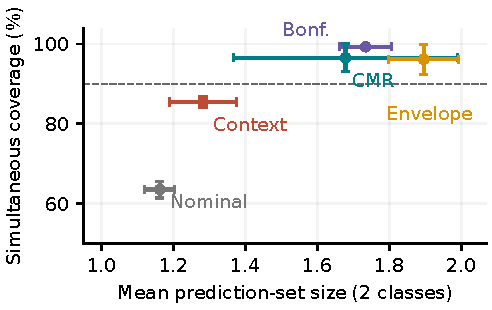
\includegraphics[width=\columnwidth]{figures/tradeoff.pdf}
\caption{Coverage--size trade-off for PneumoniaMNIST compact residual models. Points are five-seed means, bars are seed SD; size averages over queries and menu contexts. The envelope's common threshold can be conservative relative to CMR.}
\label{fig:tradeoff}
\end{figure}
The 224-pixel pretrained RN18 extension has 91.0\% source-statistics accuracy. Current-batch BN gives a 44.8\% companion-induced class-flip rate; context-specific calibration yields 92.0\% mean and 83.0\% simultaneous coverage. CMR gives 93.6\% simultaneous coverage with mean set size 1.37. This extension uses its own predefined fine-tuning protocol and does not establish clinical generalization.\par
Seed-0 normalization controls on PneumoniaMNIST yield class-flip rates of CNN-BN: 19.6\% full BN, 15.4\% mixed moments, and 15.1\% first-layer-only; ResNet-BN: 45.3\% full BN, 34.4\% mixed moments, and 12.5\% first-layer-only. The fixed 50:50 moment mixture is a control, not a full TTN implementation. Complete secondary results are released, including a matched affine-intensity condition and batch sizes 8 and 32.\par
An exploratory randomized APS sensitivity \cite{aps} shares one uniform variate across each query's contexts: the PneumoniaMNIST residual model gives 83.7\% simultaneous coverage with context-specific calibration and 92.3\% with CMR (size 1.37). Deterministic APS makes CMR and the envelope return both labels on this task. Score choice therefore changes the coverage--size trade-off; all score diagnostics are released.\par
A seed-0 validation-companion sensitivity gives 92.4\% mean versus 86.2\% simultaneous coverage for the compact pneumonia residual model. These companions were used for checkpoint selection but excluded from gradient training; results for all six configurations are released.\par
Finite calibration is visible, particularly on BreastMNIST. With only 77 calibration examples, Bonferroni's requested order statistic exceeds the available sample, returning the full label set. This is the correct finite-sample convention, not a numerical failure. Realized evaluation coverage can fall below 90\% even for valid marginal methods; Fig.~\ref{fig:splits} separates this variation from a universal guarantee for each calibration split.
\begin{figure}[t]
\centering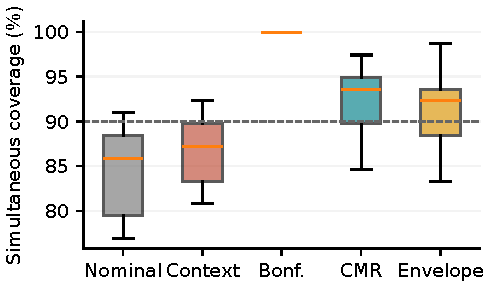
\includegraphics[width=\columnwidth]{figures/splits.pdf}
\caption{Simultaneous coverage across 100 calibration/evaluation repartitions of the fixed BreastMNIST test pool, CNN-BN seed 0. Boxes show median and quartiles; whiskers show the 5th/95th percentiles. Repartitions are dependent sensitivity trials.}
\label{fig:splits}
\end{figure}

\section{Discussion and limitations}
A calibrated service should specify whether its guarantee concerns a random realized context, each fixed context separately, or all allowed contexts for the same query. The latter can accommodate a context choice made after seeing the query, but only within the fixed, independently chosen menu. Our menu is a reproducible stress test, not an exhaustive hospital scheduler model. Protection against arbitrary companions does not follow.

A practical application is quality assurance for imaging inference services: replay unchanged studies under allowed batch compositions, measure paired prediction-set changes, and test whether reported coverage matches its stated estimand. Commercial utility, clinical benefit, patentability, and regulatory readiness remain untested.

Most experiments use compact 28-pixel models; the 224-pixel extension uses one ImageNet-pretrained backbone. Diagnostic-resolution images and medical foundation models require separate evaluation. Missing patient identifiers prevent patient-level independence claims; dermatology metadata establish lesion separation only. Global coverage can conceal rare-class failures, and benchmark labels are not independently adjudicated diagnoses. Five seeds quantify training variability, not population diversity. The bootstrap conditions on fitted models and calibration. The exploratory protocol, small breast evaluation set, and hand-designed menu limit generalization. Patient-disjoint, multisite studies and gradient-based adaptation remain future work. Our conclusion is limited to measurable companion-induced differences between ordinary and simultaneous coverage.

\section{Compliance with ethical standards}
No institutional ethics approval or waiver was obtained for this independent secondary analysis. This computational benchmark reuses public, de-identified image releases under their stated licenses: CC BY 4.0 for PneumoniaMNIST and BreastMNIST, and CC BY-NC 4.0 for DermaMNIST-C/HAM10000-derived images. No source images are redistributed with the software. The dermatology experiments do not establish permission for commercial use of the underlying data. Predictions are research outputs and are not offered as clinical decisions.

\section{Acknowledgments}
No external funding was received. The author reports no relevant financial or nonfinancial interests. OpenAI Codex (GPT-6-based assistant) was used for literature discovery, study design, software implementation, computational experiment execution and analysis, drafting Sections 1--6 and the bibliography, and generating figures and tables from saved results.

\bibliographystyle{IEEEbib}
\bibliography{references}
\end{document}
